\documentclass[12pt, english, NoHyper]{AE4010-template}
\usepackage[]{natbib}
% \usepackage[sorting=none, citestyle=numeric-comp, natbib=true]{biblatex}    % For numbered biblatex references
%  \usepackage[citestyle=authoryear]{biblatex}      % For author year biblatex references
\usepackage{csquotes}
\usepackage{hyperref}
\usepackage{amsmath}
\usepackage{graphicx}


%% Uncomment the following three lines when using the biblatex package
%\bibliography{bibliography.bib}
%\addbibresource{bibliography.bib}
%\bibliography{apa}
%% Uncomment the following line when using the natbib package
\bibliographystyle{plainnat}





%% Define your title entries here
\title{Identification of Potentially Hazardous Asteroids}
\author{J. G. P. Vermeulen}
\yourstudynumber{4382889}
\yourmscprofile{Space Flight}
\yourmsctrack{Space Systems Engineering}









%   ########################################################################
%               PLEASE COMPILE USING XELATEX FOR THE BEST RESULTS
%   ########################################################################









\begin{document}
\maketitle

\section*{Executive Summary}
In this section try and state, in under 300 words, the major aspects of your project plan. It should include what the project is about, what the main content of the plan will be what the main objectives of your research are, the methods you will use to achieve those objectives and what your possible findings could be. End with a strong sentence that highlights the significance of the work to be undertaken and any long-standing contribution to the body of knowledge. Remember that this is a proposal of work to be done and so you might also say something about the motivation and feasibility.





\section{Introduction}
In recent years, human efforts have catalogues all very large near-Earth asteroids and determined none of these to be a threat in the foreseeable future. However, as illustrated by recent impacts such as the Chelyabinsk and Tunguska meteors, smaller, unknown, asteroids still pose a significant threat to human life and property. In addition, an upscaling of Earth-based detection methods will not suffice to safeguard humanity from these natural disasters: unfavorable phase angles and atmospheric interference make detection from the Earth inefficient (\cite{DefendingPlanetEarth}). In recent years, a multitude of studies (e.g. \cite{NEOSDT1}, \cite{ThesisOlga}) have been performed to assess the effectivity of a future space-based Near-Earth Object surveying mission. These studies have yielded promising results, but still suffer from some additional issues, such as interference my sunlight and limitation on data processing. Therefore, a system of detection is proposed based on autonomous satellites placed strategically in the solar system to automatically detect near-Earth asteroids and identify whether these are impact-hazardous to Earth. \\

This work contains a project plan for proposed research into the topic of multi-satellite asteroid surveys. Firstly, an overview of the current state of literature, and the position of the work therein is discussed. Next, the core of the research as intended is described, starting with the research question, aim and subgoals; followed by the methodology, setup of the experimentation, and expected outcomes. Lastly, a short discussion of the project plan will be given.







\section{State-of-the-art/Literature Review}
Study of Potentially Hazardous Asteroids (PHA's) began through initiatives from governments to safeguard Earth from the threat of asteroid impacts, resulting in several of the foundations of the field (\cite{InitialTaskforce}, \cite{DefendingPlanetEarth}). These agreed upon the initiative to identify 90\% of all Near-Earth Asteroids\footnote{Defined as an asteroid with perihelion < 1.3 AU} larger than 140 m in diameter. This was based on the calculation that this would eliminate 90\% of the remaining background risk. Thus, the PHA was defined as an asteroid with a diameter over 140 meter, which intersects Earth's orbit within 0.05 AU. \\

In the following years, a multitude of surveys were carried out to achieve this goal, such as, but not limited to, the Catalina Sky Survey and the PANSTARRs survey in Hawaii. In addition, several surveys were carried out from space, most notable the NEOWISE survey which repurposed the WISE imager after its main cryogenic payload had run out. The performance of these surveys has been spectacular (see e.g. \cite{NEOWISEFlex}). However, as shown by \cite{PopulationHarris} in \autoref{fig:populationdifference}, a large fraction of asteroids is still unknown.\\

\begin{figure}[thb]
 \centering
 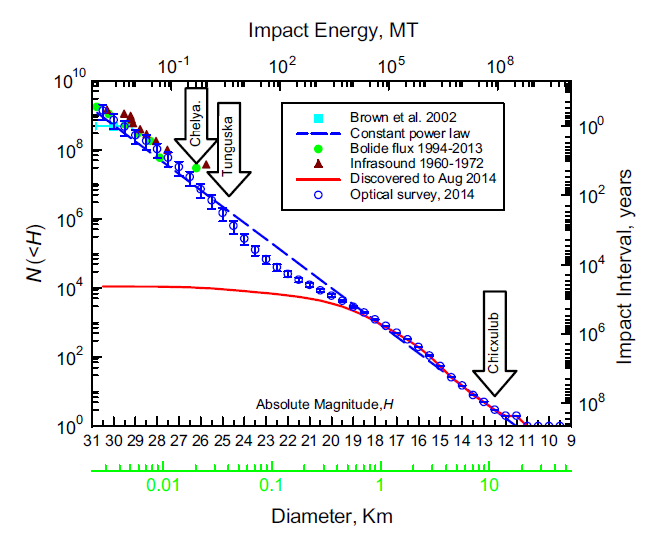
\includegraphics[width=0.8\textwidth]{figures/populationdifference.png}
 \caption{Relationship between asteroid absolute magnitude (and thus size, and impact energy) to their occurence. Shown are the expected population of these asteroids, compared to the number discovered in contemporary surveys.}
 \label{fig:populationdifference}
\end{figure}

As the remaining fraction of asteroids not only poses a threat to human safety and property, but discovering them will also yield valuable scientific insights into the structure and origin of our solar system (\cite{Populations}), a number of new surveys is currently being researched and developed. Among the ground-based surveys, the most impressive project is the Large Synoptic Survey Telescope at the Vera C. Rubin observatory in Chile (see \cite{LSST} for a thorough overview). However, as Earth-based surveys are limited by weather, day/night cycles and atmospheric dispersion, most of the research is focussed on space-based surveys. \\

Although the efficacy of Earth-orbiting missions has already been shown by missions such as the Spitzer space telescope and NEOWISE, there is currently a lot of interest in deep space surveys. Advantages of these surveys include not being influenced by sunlight reflected off Earth, more favourable viewing angles, and greater relative motion to the asteroids (\cite{NEOSDT1}). The largest barrier to performing these missions, the lack of sufficient computational power, has been resolved by advances in semiconductor technology. However, because of the vast costs of a space mission, most work is currently focussed on simulating surveys to determine optimal conditions, such as the work done at the European Space Agency by \cite{Flyeye} and at NASA Jet Propulsion Laboratory by \cite{NEOSDT2}. \\

Investigation of the possibilities yields that space-based surveys will be superior the current Earth-based surveys. Commonly researched orbits are Earth-Sun L1, Venus-Sun L1, Venus-trailing, and several Earth orbits, using either visual light or thermal infrared telescopes. \cite{ThesisOlga} expands on thes even further by showing advantages of using solar sails for more complex orbits. Although the performance of these surveys is impressive, there is still a large number of PHAs that will not be found by these surveys, and an even larger fraction of smaller NEOs that will remain undiscovered, as shown by \cite{NEOSDT2} in \autoref{fig:surveycompleteness}. Therefore, in this report, a proposal will be made to research if the performance of these surveys can be improved through utilization of a system of several satellites, hoping to exploit a greater variety in orbits, payload combinations, and viewing angles.

\begin{figure}[thb]
 \centering
 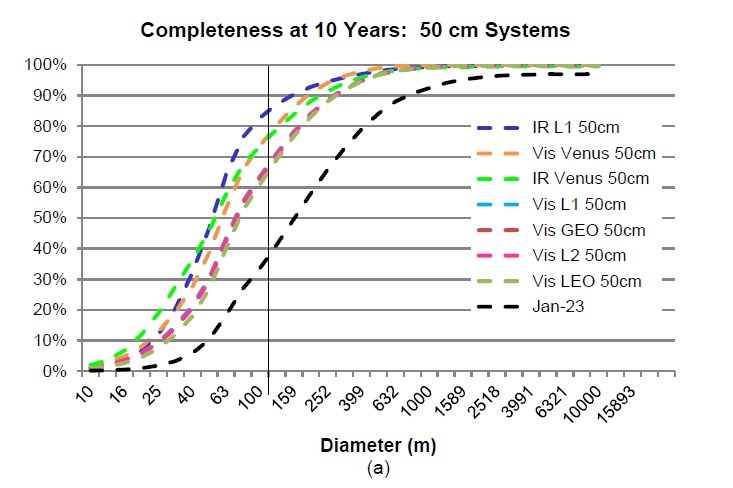
\includegraphics[width=0.8\textwidth]{figures/surveycompleteness.png}
 \caption{Survey completeness at 10 years, using 50cm telescopes.}
 \label{fig:surveycompleteness}
\end{figure}


\section{Research Question, Aim/Objectives and Sub-goals}
This section consists out of two main parts: the research questions and the research objective.



\subsection{Research Question(s)}
What is the main research question to be solved in reaching the project goal? There can be more than one but be focused. Split the research question into sub-questions, with each sub-question having further questions. The lower level questions will, together, provide the answer to the higher-level questions. These research questions should be very precise and like a requirement, be unambiguous, unique, measurable, and answerable in a meaningful way. 



\subsection{Research Objective}
The objective is basically the project goal, again clearly stated in terms of what the researcher wants to achieve, and by which means you will achieve this. Ideally formulated in the form of: \newline

\noindent The main research objective of this thesis is:

\begin{quote}
“To achieve (a) by means of(b)”.
\cite{Verschuren}    
\end{quote}


\noindent This is then followed by tangible sub-goals that will be necessary to make this happen. These sub goals can then be developed into task blocks in the project plan/Gantt chart which you are required to include in the plan later on. 





\subsection{Some tips:}
Do try and avoid using bullet lists. Objectives are not synonym for a to do list. Make the novelty and innovation of your work clear! Again, remember that this is a proposal of work to be done and so you might also say something about the motivation and feasibility. You do not need to include a research framework as part of the deliverable although you may want to create one to assist you in creating your research objective and research questions.





\section{Theoretical Content/Methodology}
What is the theoretical basis of the work to be undertaken? Refer to literature in which theory, framework or methods are explained here. Are there hypotheses to be tested? If so list them. Are a couple of theoretical approaches going to be used together in a hybrid approach? What are the steps to be undertaken in the project – linking to the objective ad research questions established in Section 3 without it resulting in a bullet list.





\section{Experimental Set-up}
What is your laboratory set-up or in the field set-up? Present it such that readers can better informed and critical of any limitations of your research environment and your set-up. For example, how will the collaboration with industry work? Or are there any practical implications of your Methodology from Section 3? Keep in mind that Experiments are more than just questionnaires, interviews or physical tests in a laboratory. Creating or modifying a computer programme or a computer model is also considered an experiment, so their set up, documentation and limitations should be discussed here. 

Do not forget to include technical details such as machines to be used, programming language or modelling software and why you selected those to reach your objective as stated in section 3.




\section{Results, Outcome and Relevance}
What data etc. will you be working with, which variables and parameters, and what type of results do you want to investigate? Then go on to try and project the sort of outcome you are interested in and of course ultimately what the relevance of that is both for your project but try and say something about possible larger impacts of your work. Mention how you expect to validate and verify your results. This is a key part of your thesis, so it is important to consider this early in your research.





\section{Project Planning and Gantt Chart}
Look at the logistics of carrying out the work, develop the intended work into work packages (from the tasks mentioned in Section 3) and then incorporate all that into a schedule of work through a Gantt chart (or Integrated Master Plan/Integrated Master Schedule). You must, at a reasonably high level, try to estimate time required and any resource constraints etc. and then fit that into a schedule. A Work Breakdown Structure and Work Flow Diagram can be very helpful (ref: DSE). You will put in three key review points: 1) the Kick-off Review/preliminary meeting; 2) the Mid-term Review; and 3) the Green Light Review. Remember holidays etc., preparing deliverables etc. and that some tasks will be concurrent and running in parallel. 

Be mindful that your planning is realistic and contains iterations and interlinking of activities to show how activities may depend on each other. Also motivate your planning, do not just put in a Gannt Chart. Use proper software to generate a Gantt chart.

\noindent Finally, the Gantt chart should visibly show any key review points, milestones (points of specific achievement relative to the end goal) and deliverables (tangible outputs such as reports, presentations, papers, manuals, tools, workshops,).






\section{Conclusions}
The conclusions regarding what you are proposing should be written in a precise, unique, clear and accurate manner. Always check if they are well supported by the work you presented in the project proposal and check them against the main literature so that you can make a statement about the longer-term impact of your work on the body of knowledge. Lift the most important conclusions into the Executive Summary and check that both are consistent, also with the Introduction. This is done because the Executive Summary, Introduction and Conclusion form the key points of entry and exit into the work and make a big impact on accessibility and getting across the relevance!

\section{References}
List all references consistently, using one of the preferred approaches, for example the Harvard referencing system. A useful link on how to quote and reference properly can be found in the Guide to Harvard referencing from the Anglia Ruskin University Library in the UK: \url{http://libweb.anglia.ac.uk/referencing/harvard.htm}. If you use numbered references do not use them as a noun and always mention the author’s name. So not: [1] says she is always right, but Saunders-Smits [1] says she is always right. Also avoid giving a lot of references in one go as in: Chocolate is a vegetable [1- 15]. Explain the view of each paper and group them per view. Now it looks like you never read all the papers and are just trying to show off.

The key thing is that the referred to author is given credit through their earlier work, that this is dated to show the chronological order of developments, and that the reader has enough information to go and find that specific reference. Relative to the latter point: where was the conference or if a journal review what was the volume or edition number and certainly page numbers. Always paraphrase or if you quote literally please use italics and quotation marks followed by the name of the author and either the year or the reference number depending on your chosen reference style to avoid even the notion of plagiarism.

The strongest references are ones that have been reviewed prior to publication (journals for example) and the weakest are web sites and popular publications. Only reputable websites (from a society or major industry player) should be included and the date of access should be noted. Preferably stay away from web references as they are so uncontrolled as sources of information especially from web fora and commercial parties.

Note: web references, lecture notes, technical reports, standard textbooks etc. do not count towards the number of quality references used as they are not scientifically peer reviewed. The number of quality references should always greatly outnumber the number of general references. It looks unprofessional to refer to the textbook and templates of this course.

Finally, when using a reference management system such as OneNote, Mendeley or BibTex, do check each entry for completeness and correctness. When filling your management system automatically, mistakes and omissions often occur. \newline


%% Use letters for the chapter numbers of the appendices. 
%% Note: when there are references in the appendices, the references should be placed below the appendices.
\appendix
%% Uncomment the following line when using the natbib package
\bibliography{bibliography.bib}

%% Uncomment the following line when using the biblatex package
% \printbibliography


\section{Gantt Chart}
Feel free to put the Gannt Chart in an Appendix. The references and the Gantt chart do not count towards the 10-page limit of the plan.

\end{document}
